\documentclass{article}

\usepackage{graphicx}
\usepackage{tikz}
\usepackage{tikzsymbols}
\usetikzlibrary{calc,patterns,shapes.geometric}
\pagestyle{empty}
\usepackage[margin=0pt]{geometry}
\geometry{papersize={14in,12in}}

\def\centerarc[#1](#2)(#3:#4:#5){\draw[#1] ($(#2)+({#5*cos(#3)},{#5*sin(#3)})$) arc (#3:#4:#5);}

\begin{document}
	\begin{figure}
		\centering
		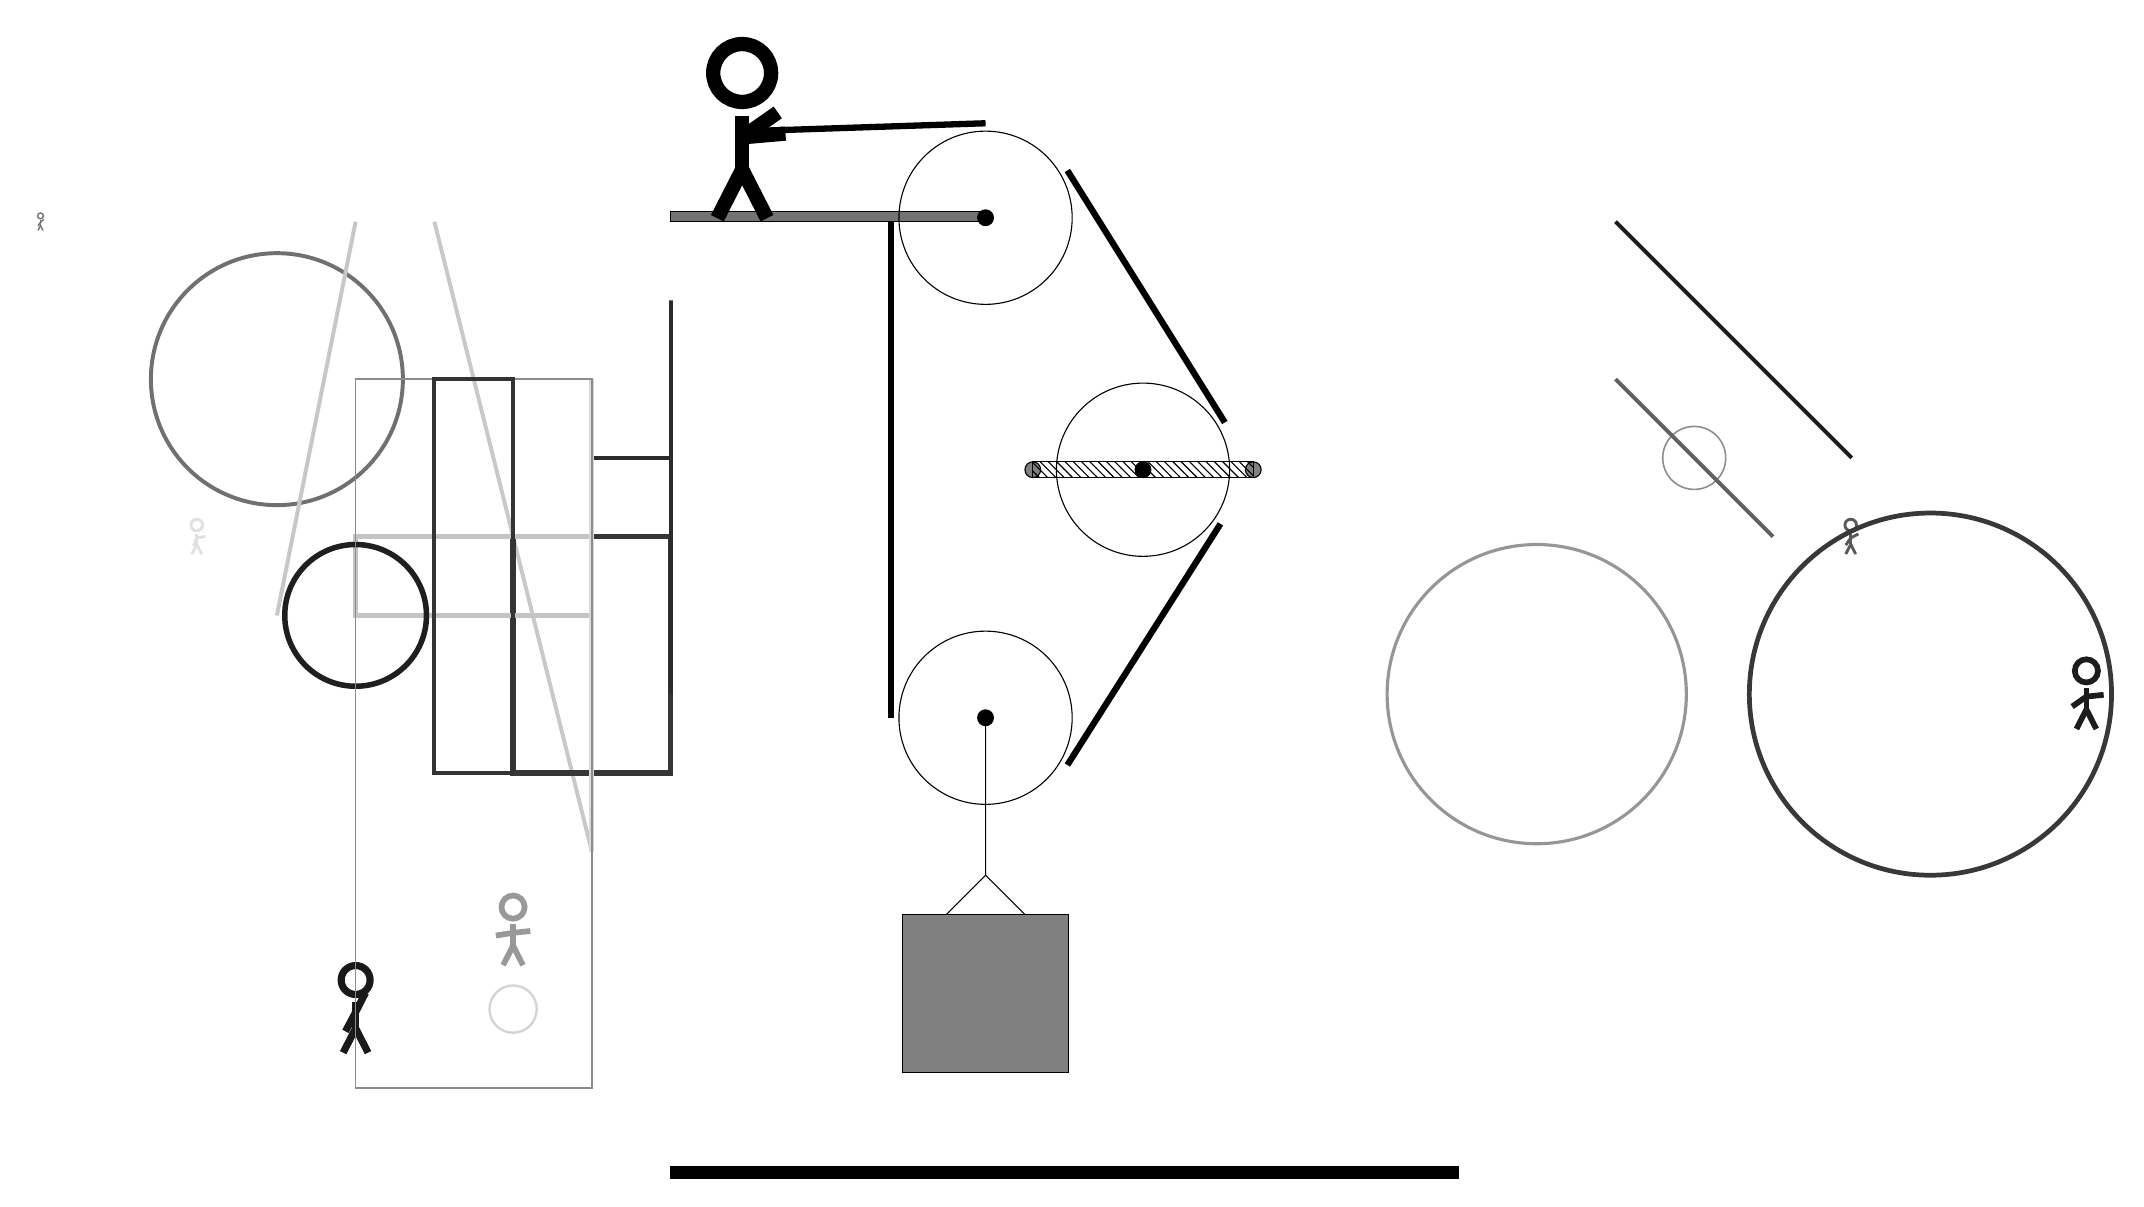
\begin{tikzpicture}
			%%%%% START %%%%%
			
			\draw[fill=black!55] (-2, 9) rectangle (2, 9.125);
			
			\draw (2, 2.7) circle (1.1);
			\draw[fill=black] (2, 2.7) circle (0.1);
			
			\draw (2, 9.05) circle (1.1);
			\draw[fill=black] (2, 9.05) circle (0.1);
			
			\draw[fill=white](4, 5.85) circle (1.1);
			\draw[fill=black] (4, 5.85) circle (0.1);
			\draw[fill=black!50] (2.6, 5.85) circle (0.1);
			\draw[fill=black!50] (5.4, 5.85) circle (0.1);
			\draw[pattern=north west lines, pattern color=black] (2.6, 5.95) rectangle (5.4, 5.75);
			
			\draw (2, 2.7) -- (2, 0.7) -- (1.5, 0.2) -- (2.5, 0.2) -- (2, 0.7);
			\draw[fill=black!50] (0.95, 0.2) rectangle (3.05, -1.8);
			
			\draw[line width=0.8mm] (0.8, 9) -- (0.8, 2.7);
			\centerarc[line width=0.8mm](2, 2.7)(180:330:1.2000000000000002);
			\draw[line width=0.8mm](3.0392, 2.1) -- (4.983, 5.1617);
			\centerarc[line width=0.8mm](4, 5.85)(390:325:1.2000000000000002);
			\draw[line width=0.8mm](5.0392, 6.45) -- (3.0392, 9.65);
			\centerarc[line width=0.8mm](2, 9.05)(30:90:1.2000000000000002);
			\draw[line width=0.8mm](2, 10.25) -- (-1, 10.15);
			
			\node at (-1, 10.15) {\Strichmaxerl[10][-175][35]};
			
			\draw[line width=0.5mm, color=black!83] (-3, 6) rectangle (-2, 2);
			
			\node[line width=0.2mm, color=black!40] at (-4, 0) {\Strichmaxerl[4][9][6]};
			\draw[line width=0.5mm, color=black!21](-3, 1) -- (-5, 9);
			\node[line width=0.5mm, color=black!89] at (16, 3) {\Strichmaxerl[4][35][6]};
			
			\draw [line width=0.2mm, color=black!45](11, 6) circle (0.4);
			\draw[line width=0.7mm, color=black!79] (-4, 2) rectangle (-2, 5);
			
			\draw [line width=0.3mm, color=black!17](-4, -1) circle (0.3);
			\node[line width=0.2mm, color=black!90] at (-6, -1) {\Strichmaxerl[5][62][63]};
			\draw[line width=0.6mm, color=black!23] (-3, 5) rectangle (-6, 4);
			\draw[line width=0.5mm, color=black!83] (-2, 3) rectangle (-2, 8);
			\draw [line width=0.5mm, color=black!56](-7, 7) circle (1.6);
			
			\draw [line width=0.7mm, color=black!88](-6, 4) circle (0.9);
			\node[line width=0.7mm, color=black!65] at (13, 5) {\Strichmaxerl[2][56][27]};
			
			\node[line width=0.7mm, color=black!12] at (-8, 5) {\Strichmaxerl[2][68][9]};
			\draw [line width=0.4mm, color=black!41](9, 3) circle (1.9);
			\draw[line width=0.6mm, color=black!15] (-3, 7) rectangle (-3, 1);
			
			\node[line width=0.2mm, color=black!55] at (-10, 9) {\Strichmaxerl[1][53][42]};
			\draw[line width=0.5mm, color=black!22](-6, 9) -- (-7, 4);
			\draw[line width=0.2mm, color=black!45] (-3, 7) rectangle (-6, -2);
			
			\draw[line width=0.5mm, color=black!89](10, 9) -- (13, 6);
			\draw[line width=0.5mm, color=black!80] (-4, 2) rectangle (-5, 7);
			\draw[line width=0.5mm, color=black!62](12, 5) -- (10, 7);
			\draw [line width=0.6mm, color=black!78](14, 3) circle (2.3);
			
			\draw[fill=black] (-2, -3) rectangle (8, -3.15);
			
			%%%%% END %%%%%
		\end{tikzpicture}
	\end{figure}	
\end{document}